\documentclass[fleqn,11pt,openany]{book}

% These two need to be set before including scirun style package
\title{Ischemia Model tutorial}
\author{Jeroen Stinstra, Darrell Swenson}

% INCLUDE SCI STYLE DOCUMENT
\usepackage{scirun}

\begin{document}

%% starting from SCIRun Doc wiki
%% http://software.sci.utah.edu/SCIRunDocs/index.php/CIBC:Documentation:SCIRun:Tutorial:BioPSE


% CREATE TITLE PAGE --------------------------------------------------
\maketitle

% CHAPTERS ---------------------------------------------------------------

\chapter{Overview}

\begin{introduction}

This tutorial demonstrates several tools within SCIRun for building models out of imaging data. 
It describes the pipeline starting from preprocessed images to generate a computational mesh and adapt this mesh to meet the computational requirements.
It then continues to set up a finite element bidomain simulation,  and demonstrates how results can be visualized.   

\end{introduction}

\section{Ischemia Model}

This tutorial describes the generation of a quasi-static volume conductor model of an ischemic heart based on data from actual experiments.
The goal of this modeling pipeline is to generate experiment-specific models of the myocardium.
The MR images that will be used in this example have been derived from a dog heart that was scanned to obtain anatomy, fiber orientation and the perfusion bed of left anterior descending artery.
The goal of the simulations is to render a model that can be used to predict extracellular cardiac potentials as measured by electrodes onto on an isolated heart or with needles inserted into the heart. 

The background behind this research is to provide insight into the question how reduced flow or additional load affect regional acute ischemia. By measuring many anatomic details and electrical measurements we hope to provide insight in what is going on in the border zones between the healthy and ischemic tissue layers. This tutorial describes one specific aspect of that research namely the creation of a forward model of ischemia based on measured anatomical data such as muscle fiber orientation and perfusion beds of the coronary arteries.

The electrical model that is described in this tutorial is a so called bidomain model. In the bidomain model one assumes that all electrical sources within the heart are located within the cell membranes of myocytes (heart cells). As the intracellular electrolytes of all the myocytes are connected to each other by means of  gap junctions (a protein that connects the insides of two cells together), the intracellular and extracellular spaces can be assumed as two continuous spaces that are separated at each location by a cell membrane. 

During the plateau phase of the action potential all cells can be assumed to be in a depolarized state, however the transmembrane potential (the potential difference between the intracellular and extracellular space) is not the same for ischemic and healthy cells. The latter effect causes so called injury currents to flow within the intracellular and extracellular spaces. These currents can be observed at the surface of the heart as potential differences that translate to so called ST shifts in the ECG.   

In order to model these currents one needs a description of the electrical properties of both the intracellular and extracellular spaces. Both can be modeled as anisotropic volume conductors that have the shape of the heart and where the anisotropy is caused by the fiber structure of the myocardium (cardiac muscle tissue). The partial differential equations to solve in both spaces are the following:

\begin{eqnarray} 
	\nabla \cdot \Sigma_i \nabla \phi_i &=& i_{mem} \\
	\nabla \cdot \Sigma_e \nabla \phi_e &=& -i_{mem}
\end{eqnarray} 

\noindent where $\phi_i$ and $\phi_e$ are the intracellular and extracellular potentials respectively and $\Sigma_i$, and $\Sigma_e$ are the conductivity tensors of both spaces. Finally, $i_{mem}$ is the current through the membrane. We can define the transmembrane potential as:

\begin{equation}
  	\phi_m = \phi_i - \phi_e
\end{equation}

\noindent Combining this equation with the previous set of equations results in the system to solve being:

\begin{equation}\label{eqn:bidomain2}
	\nabla \cdot (\Sigma_i + \Sigma_e ) \nabla \phi_e = -\nabla \cdot \Sigma_i \nabla \phi_m
\end{equation}

The latter equation describes the potential of the extracellular space, as observed in measurements, as a function of the membrane potential $\phi_m$. To solve this for a specific heart, one needs to have a description of $\Sigma_i$ and $\sigma_e$ as a function of space and one needs to have a description of how $\phi_m$ changes throughout the border zone. In this tutorial we will first describe how to load the imaging data and how visualize this, subsequently this imaging data is turned into a description of $\Sigma_i$, $\Sigma_e$, and $\phi_m$, which in the final chapter then is used to solve the extracellular potential $\phi_e$.

\section{Software requirements}

\subsection{SCIRun module compatibility}

The modules demonstrated in this tutorial are available in SCIRun version 4.0 and higher and this tutorial is not compatible with any older version of SCIRun. 
Also be sure to update your SCIRun version to the latest built available from the \href{http://software.sci.utah.edu}{SCI software portal}, which will include the latest bug fixes and will make sure that the capabilities demonstrated in this tutorial are up to date.

Because this tutorial demonstrates the meshing capabilities available within SCIRun, it is necessary to obtain a version of SCIRun that includes the meshing tools (currently an interface to TetGen).
The easiest way to obtain a SCIRun version that includes these tools is to download a binary version of the software, which is available for both OS X and Windows at the \href{http://software.sci.utah.edu}{SCI software portal}. 

Unfortunately for Linux users there is no binary yet available.
Hence, to run this tutorial, one has to compile SCIRun from scratch.
Download SCIRun from the SCI software portal at {http://software.sci.utah.edu } and follow the instructions in the InstallationGuide to build SCIRun from scratch. 
The supplied build script (\textbf{build.sh}) will build SCIRun with meshing tools enabled by default.

\subsection{Required Datasets}

This tutorial relies on several datasets that are part of the SCIRunData bundle.
To obtain these datasets, please go to the \href{http://software.sci.utah.edu}{SCI software portal}, follow the {\bf Download SCIRun} link, and instead of the SCIRun source or binary files, download one of the SCIRunData zip files.
Note the latter is available as a Windows zip file or as a Linux gzip file.
Both however contain the same datasets and only one of them has to be downloaded.


%---------------------------------------------

\chapter{Reading and Visualization of Image Data}

\begin{introduction}
Scope: Finding Modules - Building Networks  - Loading Data - Visualization of 3D Datasets
\end{introduction}

\begin{figure}
\scalebox{0.5}{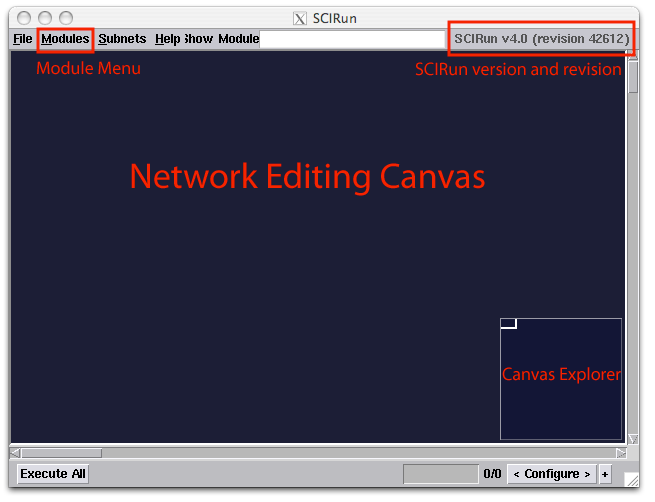
\includegraphics{IschemiaModelTutorial_figures/MainSCIRunWindow.png}}
\caption{The main SCIRun window}\label{fig:MainSCIRunWindow}
\end{figure}

\section{Loading The Dataset}

We start by opening the main SCIRun window by launching SCIRun by either double clicking on the binary icon or by launching SCIRun from the command line.
A detailed description of how to run SCIRun is given in the {\bf BasicTutorial}.
Once SCIRun has been launched the main Window with the Network editor is shown.
Figure~\ref{fig:MainSCIRunWindow} shows the main SCIRun network editor.
For this tutorial we will be selecting modules from the top menu called {\bf Modules}, this menu is used for inserting modules into the network editor.
In order to run this tutorial you need to have a SCIRun 4.x version or greater with a {\bf revision number} of {\bf 42612} or higher, the SCIRun version and revision number can be found in the upper right corner of the SCIRun editor window. 

Besides walking through the {\bf Modules} menu and finding a specific module by navigating through every submenu, a module can simply be found by typing the name of the module into Show Module entry box located in the top menu bar.
This will highlight the location of a specific module within the {\bf Modules} menu as is demonstrated in figure~\ref{fig:FindModule}. 

\begin{figure}
\scalebox{0.5}{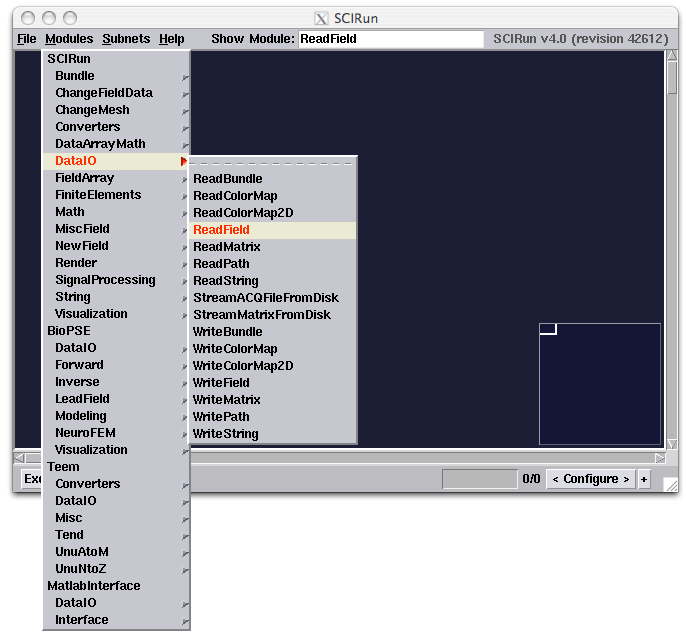
\includegraphics{IschemiaModelTutorial_figures/FindModule.png}}
\caption{Finding a module}\label{fig:FindModule}
\end{figure}

Enter \enquote{{\bf ReadField}} in the upper menu bar and follow the highlighted menus in the {\bf Modules} menu and select the {\bf ReadField} module form the menu. This will insert the {\bf ReadField} module in the upper left corner of the network editor. This module will now be used to read in the first dataset. 

The Dataset that is used in this example is called {\bf heart-ischemia} and it can be found in the SCIRunData bundle that can be downloaded as well from the SCI software portal ({http://software.sci.utah.edu}). After downloading the SCIRunData zip file, unzip the file inside a directory and inside you will find a sub directory with the {\bf heart-ischemia} datasets. If this dataset is not available in your copy of the SCIRunData bundle, please download the latest version from the website to obtain a copy.
 
\begin{figure}
\scalebox{0.5}{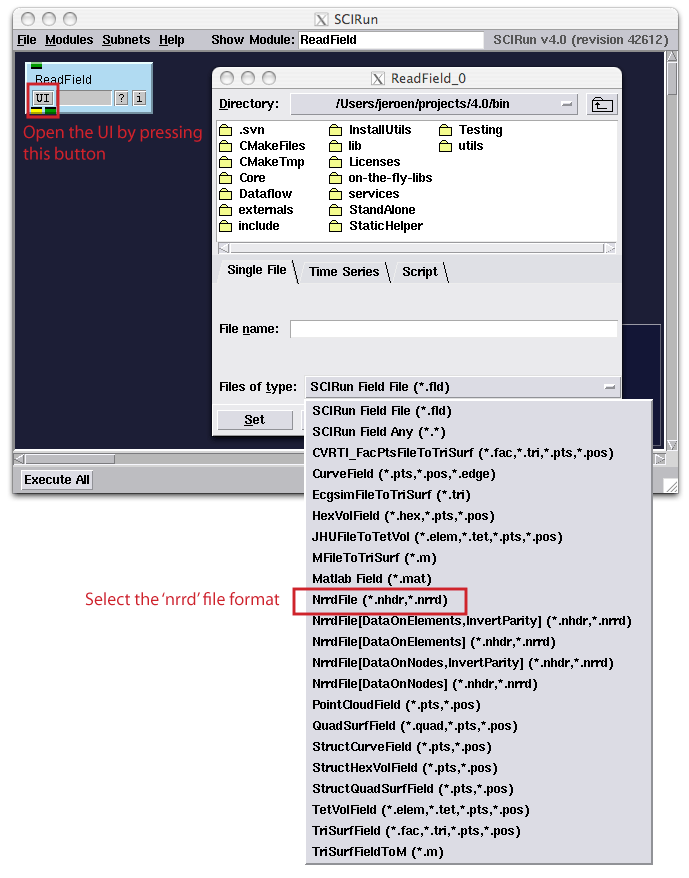
\includegraphics{IschemiaModelTutorial_figures/ReadField.png}}
\caption{Select a file name and a file type}\label{fig:ReadField}
\end{figure}

By pressing on the {\bf UI} button of the {\bf ReadField} module a browser window is opened where one can enter the name of the file that needs to be loaded. The files that are used in this example were generated by the {\bf Seg3D} software and are in the {\it .nnrd} file format. This file format is used to represent regular spaced image data, such as MRI images or segmentations. It consists of a simple text header specifying the dimensions of the data and its location in space, followed by binary data representing the actual data. This file format allows for either a header be appended to the start of the file ({\it .nrrd} format) with header and data being in one file or having a separate header file that wraps the data found in a general binary data file ({\it .nhdr} format). More information on the {\it .nrrd} format can be found at {http://teem.sourceforge.net/nrrd/format.html}.

Once the UI Window of the {\bf ReadField} module opens, select the {\bf NrrdFile} file type and use the upper part of the UI to locate the dataset by browsing the directories to the location where the SCIRunData has been saved. Open the {\bf heart-ischemia} directory and select  {\bf HeartMRI.nrrd} file. Then press {\bf Set} at the bottom of the UI to store the file name and type in the module. This process is illustrated in figure~\ref{fig:ReadField}.

Now use the Show Module menu again and find the {\bf ReportFieldInfo}. Insert this module into the network editor. Connect the two modules by clicking on one of the yellow port of either module with the middle mouse button. By dragging the connection (while pressing the middle mouse button) from the port from the first module to the second module, the two modules can be connected. Now press {\bf Execute All} to execute the modules in the network, as is illustrated in figure~\ref{fig:ReadField}. After the network has been executed, one can open the {\bf UI} of the {\bf ReportFieldInfo} module to inspect the type of data that has been loaded.

In this case the data is represented as a {\bf LatVolMesh}, the latter mesh type is used by SCIRun to represent regularly spaced data like CT or MRI data. Besides the type of data inside the pipeline, the module also shows the dimensions of the grid and the location in space derived from the original imaging data. An example of all the information displayed is shown in figure~\ref{fig:FirstNetwork}.
 
\begin{figure}
\scalebox{0.5}{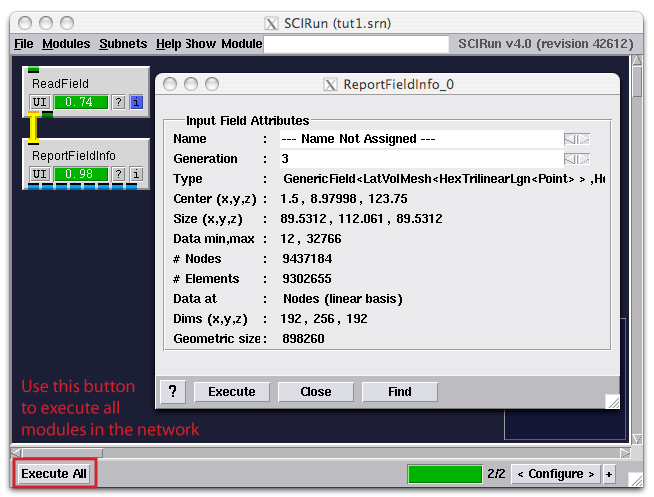
\includegraphics{IschemiaModelTutorial_figures/FirstNetwork.png}}
\caption{Network for checking contents of the file}\label{fig:FirstNetwork}
\end{figure}
 
\section{Visualization of Dataset}
 
Now we have the data loaded into SCIRun, we can actually visualize the 3D image dataset. Because we do not need the {\bf ReportFieldInfo} module for the next part of the tutorial we can delete the module from the network. Destroy the {\bf ReportFieldInfo} module by clicking on the module with the right mouse button. This will show a menu, select {\bf Destroy} from the menu and the module will be deleted from the network editor.  
 
To visualize the 3D dataset we convert the module into a 3D texture object, which will allow us to quickly browse through the dataset. Use the Show Module feature in the menu bar to insert the following modules {\bf ConvertFieldsToTexture}, {\bf ShowTextureSlices}, {\bf CreateStandardColorMaps}, {\bf ShowScene} and connect the modules as depicted in figure~\ref{fig:FullNetwork}. Note that not the full name needs to be entered each time in the Show Module text field: if a part of a module name is entered all the modules that match that part of the name will show up. This can be useful to search for new modules that for instance operate on a Field ({\em e.g.} by typing Field).

After the network of figure~\ref{fig:FullNetwork} has been entered in the Network Editor, open up the {\bf UI} of the  {\bf ShowTextureSlices} module and select to show the X, Y, and Z plane as indicated in the figure. Now execute the network. The resulting visualization is now located in the ViewScene module, press the {\bf VIEW} button of the module to see the visualization.

\begin{figure}
\scalebox{0.5}{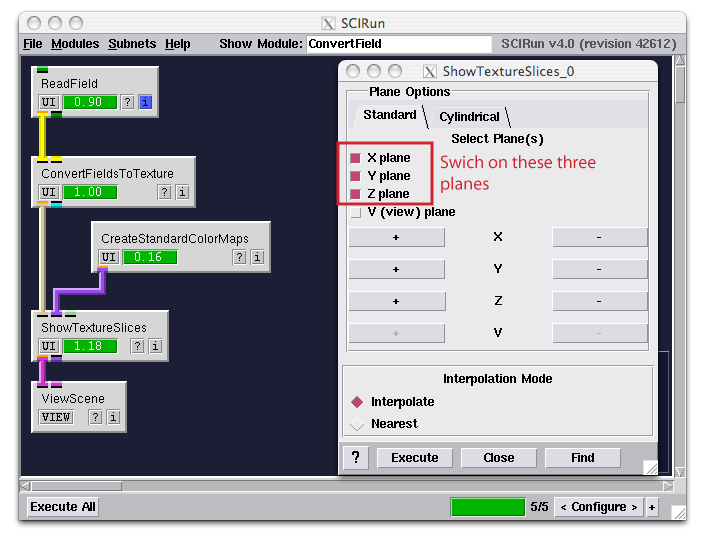
\includegraphics{IschemiaModelTutorial_figures/FullNetwork.png}}
\caption{Network for checking contents of the file}\label{fig:FullNetwork}
\end{figure}

When the ViewScene Window depicts a black space after it has been opened, press {\bf Autoview} in the viewer to ensure that the viewer is looking at the loaded data set. Once {\bf Autoview} has been pressed the resulting dataset should look like the image depicted in figure~\ref{fig:FirstViewer}. By pressing {\bf Shift} and clicking with the left mouse button on the light blue widget in the center of the viewer, the currently visible plane of the of 3D dataset can be altered. 

\begin{figure}
\scalebox{0.5}{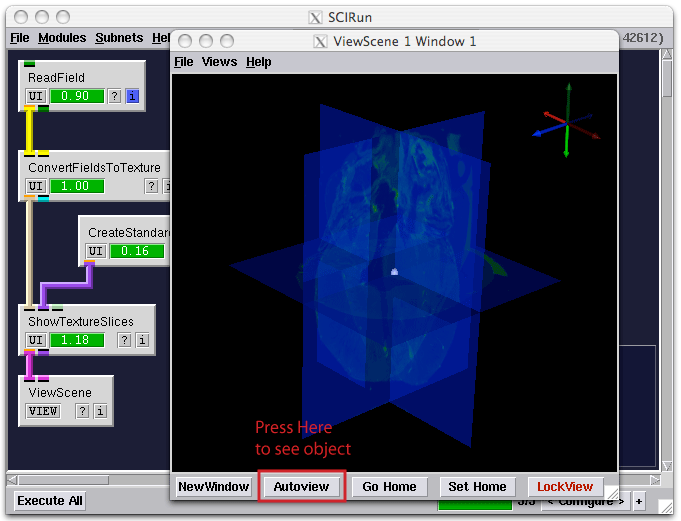
\includegraphics{IschemiaModelTutorial_figures/FirstViewer.png}}
\caption{Network for checking contents of the file}\label{fig:FirstViewer}
\end{figure}

By clicking on the {\bf UI} of {\bf GenerateStandardColorMaps} module, the colormap of the current visualization can be altered (illustrated in figure~\ref{fig:ChangingColorMap}). The transparency of the colors can be edited by clicking on the red line in the center of the colorbar. When the line is at the top the color is opaque and when the color is at the bottom the color is transparent. Try to make the background transparent. The slider just below that controls where the largest gradient in color should occur by sliding it to the left a higher contrast is generated. In the lower part of the menu one can now select from a series of predefined colormap lookup tables to alter the appearance of the image.

\begin{figure}
\scalebox{0.5}{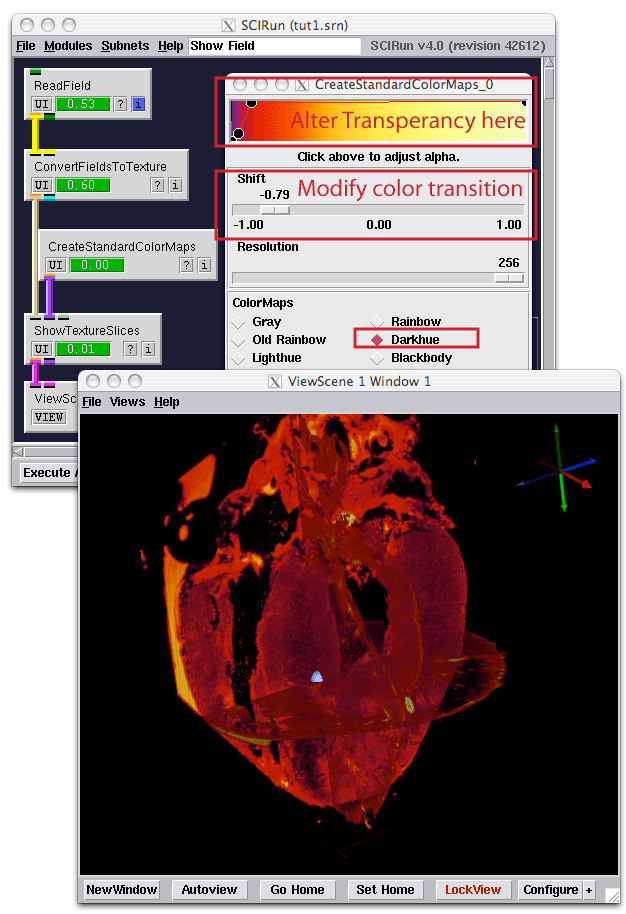
\includegraphics{IschemiaModelTutorial_figures/ChangingColorMap.png}}
\caption{Network for checking contents of the file}\label{fig:ChangingColorMap}
\end{figure}

%---------------------------------------------

\chapter{Visualization of Image Data}

\begin{introduction}
Scope: Volume Renderer - ViewScene Module - Resampling - Rendering Glyphs - Calculator Module
\end{introduction}

\begin{figure}
\scalebox{0.5}{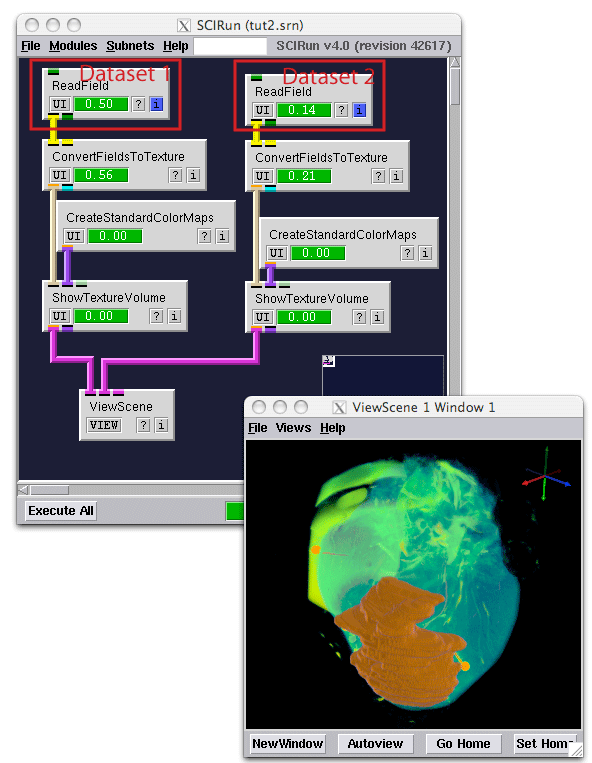
\includegraphics{IschemiaModelTutorial_figures/TwoDataSets.png}}
\caption{Reading in two datasets}\label{fig:TwoDataSets}
\end{figure}


\section{Volume Renderer and Clipping Planes}

In the previous chapter one dataset was explored, however the SCIRun viewer is capable of rendering many datasets in the same viewer, so one can explore the correlation between the data or combine them to build a model. In the next example we will be loading two datasets into the viewer. To do this we start with a similar network as depicted in the previous example. However instead of viewing slices we will use the {\bf ShowTextureVolume} module to volume render multiple datasets into the viewer. This module requires the same inputs as the {\bf ShowTextureSlices} module, but now renders the full volume transparent.

\begin{figure}
\scalebox{0.5}{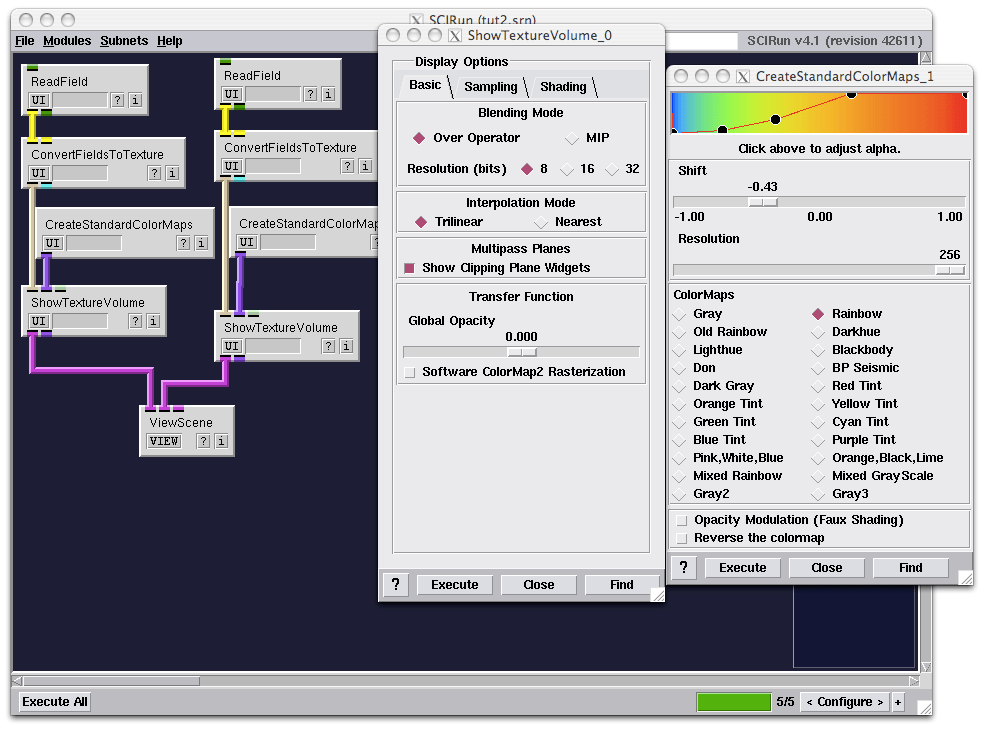
\includegraphics{IschemiaModelTutorial_figures/VisParameters.png}}
\caption{Reading in two datasets}\label{fig:VisParameters}
\end{figure}

Create the network shown in Figures~\ref{fig:TwoDataSets} - \ref{fig:VisParameters}  , and use the {\bf HeartMRI.nrrd} and {\bf HeartMRI-Perfusionbed.nrrd} as the two datasets for the two {\bf ReadField} modules. Once the network executes the data of the two datasets is combined into one visualization of the data. Try to alter the transparency of the colormaps to highlight the needle markers that were inserted into the heart and the perfusion bed of one of Left Anterior Descending Artery. An example of such a visualization is given in figure~\ref{fig:TwoDataSets}.

\begin{figure}
\scalebox{0.5}{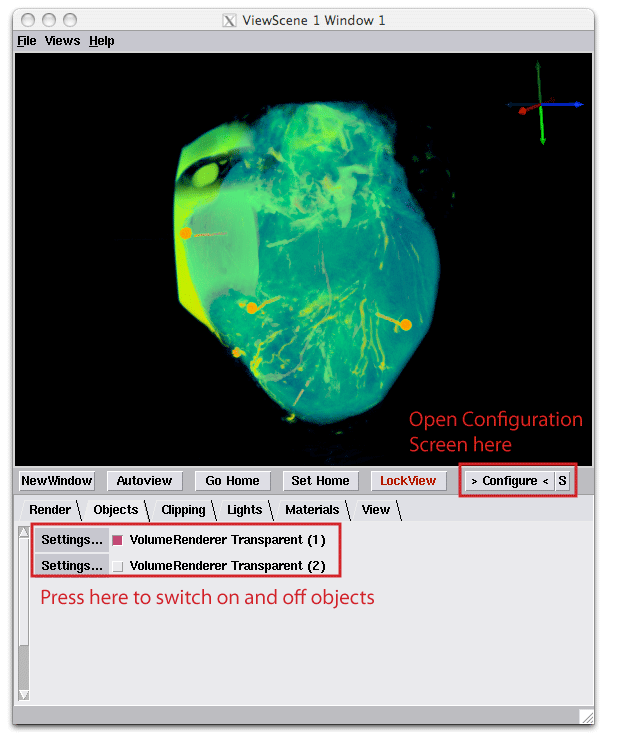
\includegraphics{IschemiaModelTutorial_figures/ViewerOptions.png}}
\caption{Opening the configuration tray}\label{fig:ViewerOptions}
\end{figure}

The datasets in this example originate from an isolated dog heart in which the Left Anterior Descending Artery was perfused with Gadolinium preparation so it shows up in an MR scan. The  heart was subsequently scanned to generate an anatomical image of the heart  {\bf HeartMRI.nrrd} and a diffusion tensor image (DTI) {\bf HeartMRI-FiberOrientation.nrrd}. Using the {\bf Seg3D} program the ventricular myocardium and the perfusion bed were segmented out of the anatomical image ({\bf HeartMRI-Segmentation.nrrd} and {\bf HeartMRI-PerfusionBed.nrrd}).

\begin{figure}
\scalebox{0.4}{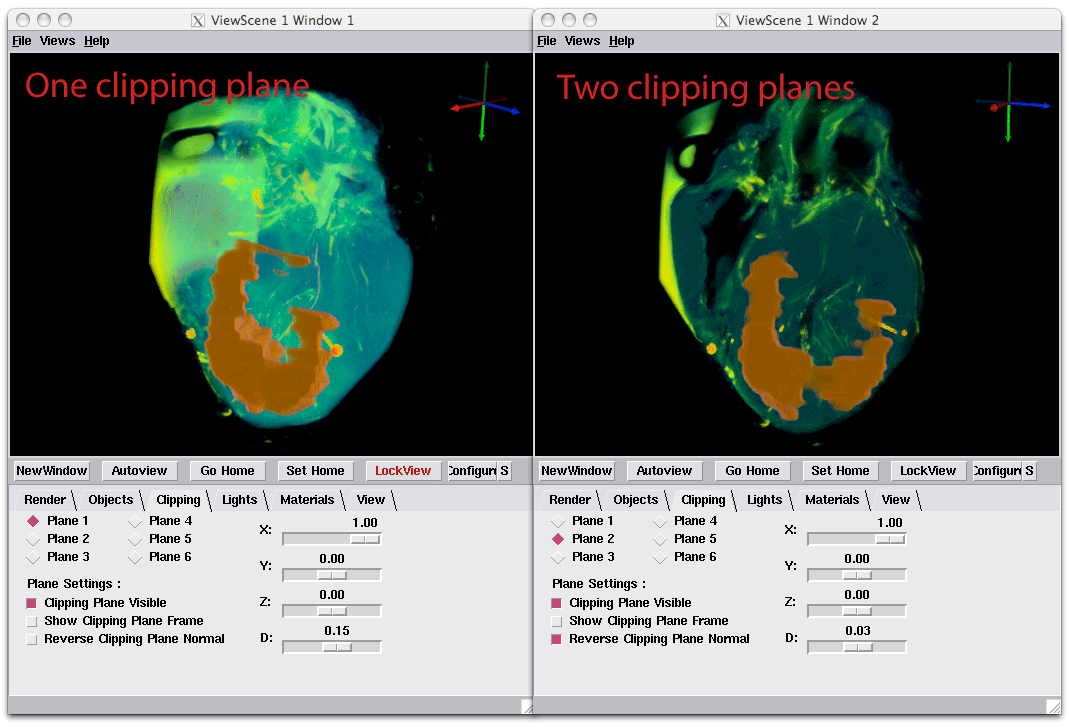
\includegraphics{IschemiaModelTutorial_figures/SlicingExample.png}}
\caption{Slicing the dataset}\label{fig:SlicingExample}
\end{figure}

Although displaying the two datasets into one image is useful, one does not always want to see each component of the data. To edit what is actually displayed in the image, open up the {\bf ViewScene} module and press {\bf Configure}. This will add a tray below the current window, with different tabs to edit different aspects of the image.  Select the {\bf Objects} tab. This tab shows the current components displayed in the view window. Pressing  selection buttons as highlighted in figure~\ref{fig:ViewerOptions} will switch on and off the displaying of a certain component.

Also try the {\bf Clipping} tab, which will allow to clip the visualization. Open up the {\bf Clipping} tab and switch on the {\bf Clipping Plane Visible} button, next drag the {\bf X} slider to 1.0. Now use the {\bf D} slider to slide the clipping plane along the X-axis. The clipping widget has been configured, so that {\bf D} corresponds to the full range of X that is spanned by the two images that are displayed in the viewer window. By dragging {\bf D} from -1 to +1 one can slice the full rendering. An example of such a visualization is depicted in figure~\ref{fig:SlicingExample}. The figure on the left shows the result of one slicing plane, the result on the right shows two slicing planes. To activate the second slicing plane, press {\bf Plane 2} and then activate this plane by selecting the {\bf Clipping Plane Visible} once more. To make it easier to generate a thin slice, select the the {\bf Reverse Clipping Plane Normal} option for the second clipping plane as this reverse the visible part of the image. By lining up the two clipping planes one can generate a small thin slice. 

If the slice becomes too transparent, open up the {\bf UI} of the {\bf ShowTextureVolume} module. One of the main options is the Global Opacity. Changing this slider the volume rendered object can be made more or less transparent. 

\begin{figure}
\scalebox{0.5}{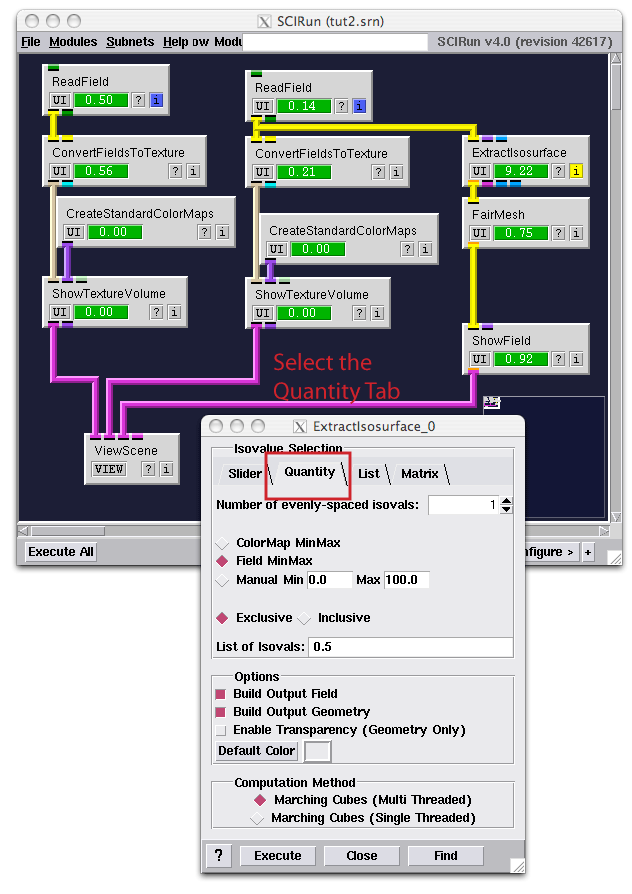
\includegraphics{IschemiaModelTutorial_figures/ExtractIsoSurface.png}}
\caption{Extracting an Isosurfacet}\label{fig:ExtractIsosurface}
\end{figure}

\section{Isosurfacing and Mesh Fairing}

In order to build a model out of the datasets we need to translate the volumes into parametric surfaces. One way to do this is to generate an isosurface. Modify the network by adding the {\bf ExtractIsosurface}, {\bf FairMesh} and {\bf ShowField} modules to the network, as depicted in figure~\ref{fig:ExtractIsosurface}. The {\bf ExtractIsosurface} should get its input from the module that reads the perfusion bed field. Make sure to select the {\bf Quantity} tab in the {\bf UI} of the {\bf ExtractIsosurface} module as depicted in figure~\ref{fig:ExtractIsosurface}. 

The {\bf ExtractIsosurface} module extracts an isosurface out of any field. In this case we are extracting it out of the segmented perfusion bed by selecting a value between the maximum and minimum value in the field. In this case the background and the segmentation have a different but constant value and hence the boundary between them will be selected. The isosurface is extracted using the Marching Cubes method which will insert an approximation of the isosurface for each element in the mesh.

The {\bf FairMesh} module takes the output from the {\bf ExtractIsosurface} module and smoothes out the surface. Because the data is discretized the isosurface will be {\em stair-stepped}. The {\bf FairMesh} module takes the surfaces and uses information about the neighborhood of the surface to generate a smoother looking surface. The resulting surface is a surface that is tessalated by triangles. Because this field is no longer structured like a regular grid, one cannot use the {\bf ShowTextureVolume} to display the surface. Instead we use the  {\bf ShowField} module that is a general module for visualizing any field. The output of this module can again be displayed into the {\bf ViewScene} module, which now combines visualizations of all three modules.

\begin{figure}
\scalebox{0.4}{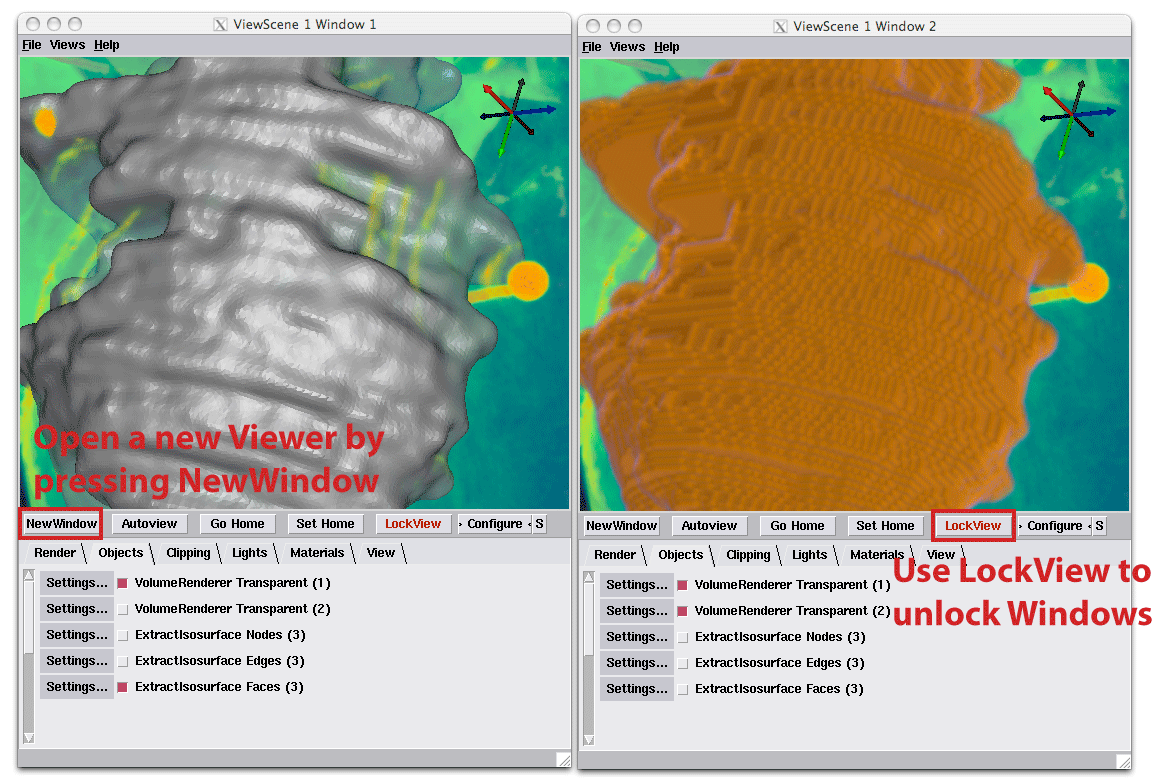
\includegraphics{IschemiaModelTutorial_figures/TwoViewers.png}}
\caption{Coupling Two ViewScene Windows}\label{fig:TwoViewers}
\end{figure}

To compare the volume rendering against the smoothed surface model, the {\bf ViewScene} module has the option to display two coupled Viewer windows. Open up the Viewer window from the {\bf ViewScene} module. Press the {\bf NewWindow} button to generate a similar ViewScene window with the same dimensions. Now open up the configuration tab on both windows. By selecting different objects in both windows, the windows can be customized to display a different aspect of the Scene. Display the Faces of the Isosurface in one window and the volume rendering of the VolumeRendering in the other window to examine the difference between the two visualizations, as depicted by figure~\ref{fig:TwoViewers}.

By zooming in into the model of the surface one can see the difference between the two renderings. Note that by default the two windows are locked together. Meaning that rotations in one window are automatically applied to the other window. This option allows to highlight the same spot in space in both windows without the need to actually align both images manually. This option can however be switched off. Press the {\bf LockView} button to unlock the window. When pressing the button the {\bf LockView} button changes color to indicate that it is switched off. One can now independently orient the windows. Locking the windows together again will not align the windows but keep the relative change between the windows. The changes are however applied to both windows. To align the windows again select the {\bf Views} menu at the top of the window and select the {\bf Other Viewer Windows} menu and select the option to get the view from the other window. This will align the view to the view of the other window. 

Locking can also be activated by pressing {\bf L} on the keyboard when the window is selected. Likewise a view from an other window can be copied by pressing {\bf ctrl 1} to copy the view from the first window, {\bf ctrl 2} for the second window and so on. The viewer also as predefined views along the axis that can be accessed by pressing {\bf 1 - 8} on the keyboard. Autoview also has a keyboard shortcut and is activated by pressing {\bf 0}. 

\begin{figure}
\scalebox{0.6}{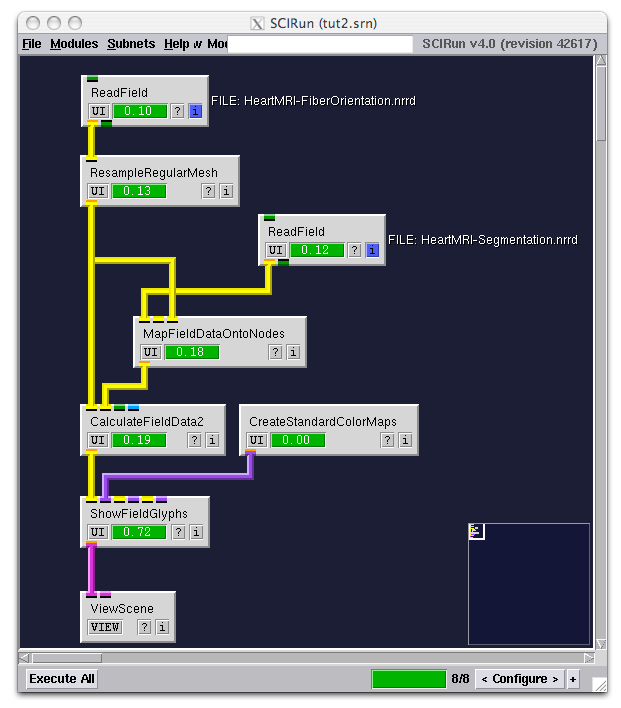
\includegraphics{IschemiaModelTutorial_figures/VectorNetwork.png}}
\caption{Network for Visualizing the Fiber Orientation of the Data}\label{fig:VectorNetwork}
\end{figure}

\section{Resampling and Viewing Glyphs}

After viewing perfusion bed, the other data to explore is the fiber orientation. Fibers cannot easily be volume rendered as the data are not scalar, but are in fact vectors. This data was derived from the Diffusion Weighted Images by doing a decomposition of the tensor and extracting the dominant direction from the data. This data can however still be loaded using the {\bf ReadField} module and the data will be translated into a LatVolMesh again, however this time the data located at each node is a vector instead.

In order to visualize the vector data we use the network depicted in figure~\ref{fig:VectorNetwork}. This network adds the following new modules to the network: {\bf ResampleRegularMesh}, {\bf MapFieldDataOntoNodes}, {\bf CalculateFieldData2}, and {\bf ShowFieldGlyphs}. 

The {\bf ResampleRegularMesh} module resamples the data. Its default settings downsample the data by a factor 2 in each direction. This module has been added here to ensure that the network executes relatively fast and that the visualization is not clobber by a huge amount of vectors. The default settings in the UI of this module should do for demonstrating displaying vectors.

Because the Diffusion Tensor Image was recorded at a different resolution as the anatomical MR image, the data in the segmentation which was derived from the anatomical scan is not in the same grid as the vector data. We apply the  {\bf MapFieldDataOntoNodes} to map the data from the segmentation onto the mesh of the Diffusion Tensor Imaging data. The module operates by looking up the value of the data in the segmentation for node in the mesh of the Diffusion Tensor Image. The result is a field that has the segmentation projected onto the same grid as the vector data.

The mapped segmentation can now be used to mask out any data that is located outside of the heart. In order to mask the data we use the general purpose calculator module, called {\bf CalculateFieldData}. There are currently three versions of this module available called  {\bf CalculateFieldData}, {\bf CalculateFieldData2}, and {\bf CalculateFieldData3}. The sole difference between these modules is the number of field input ports. As in this case we want to use two fields as input we use the {\bf CalculateFieldData2} module.

\begin{figure}
\scalebox{0.5}{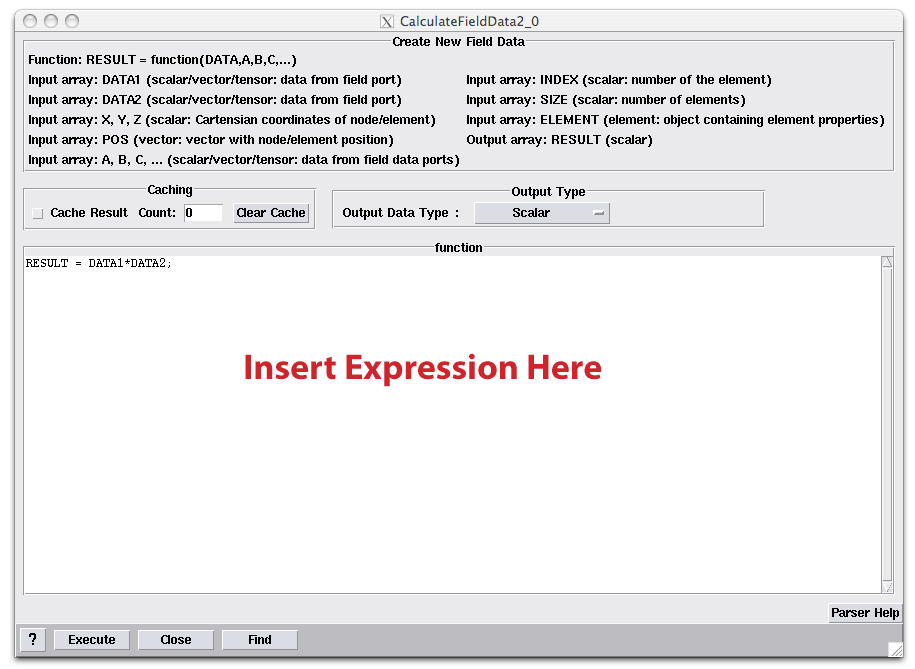
\includegraphics{IschemiaModelTutorial_figures/CalculatorModule.png}}
\caption{The UI of The CalculateFieldData2 Module}\label{fig:CalculatorModule}
\end{figure}

The {\bf CalculateFieldData2} operates by taking data from the two input fields as two input streams and applying the operation specified inside the {\bf UI} of the module to each pair of data from the two fields, as depicted by Figure~\ref{fig:CalculatorModule}. Hence, this module defines an operator that works on a stream of input data. In this case specify the input function as {\em RESULT = DATA1 * DATA2; }. In this formula {\em DATA1} is the data from the first field and {\em DATA2} is the data from the second field. As the segmentation defines the outside by a value zero and the inside as a value one, this expression masks the data and will generate vectors of zero length outside of the heart and keeps the input vector value for the vectors inside the heart. 
 
\begin{figure}
\scalebox{0.4}{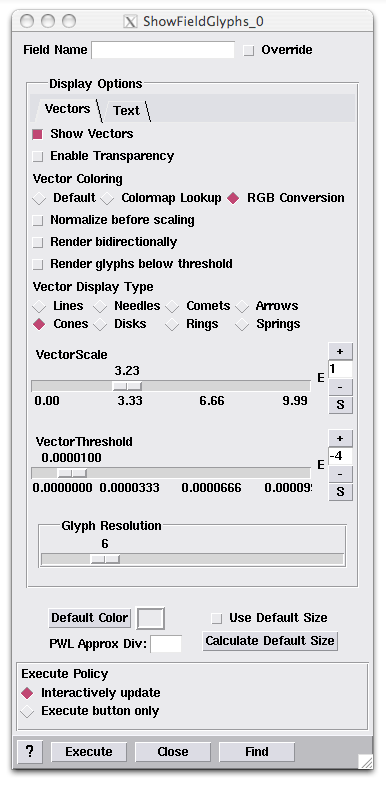
\includegraphics{IschemiaModelTutorial_figures/ShowFieldGlyphs.png}}
\caption{The UI of the ShowFieldGlyphs Module}\label{fig:ShowFieldGlyphs}
\end{figure}
 

The {\bf CalculateFieldData2} defines a whole range of mathematical operators that can be applied to a fields and a range of possible input streams that range from the location of nodes to the data values located in the field. To obtain more information on the actual operators that are available for this calculator module press the {\bf Parser Help} button in the module. This opens a document describing the expression language that has been integrated into SCIRun.  Note that the module has build in logic to determine the output type, even though the output type is set to Scalar it will in fact render a Vector output. The {\bf Output Data Type} in the latest version of SCIRun is thence no more than a hint of what output type would be preferred. In most cases the user should not need to set an output type, only when for memory reasons the data should be different from a double precision representation, this type should be set. 
 
Finally the {\bf ShowFieldGlyphs} allows for displaying the vectors in the viewer (see figure~\ref{fig:ShowFieldGlyphs}). This module is primarily used to display Vectors or Tensors that are located inside a field. As this module takes many different inputs, one needs to execute the module before one can select displaying Vectors. The reason for this is that the module first needs to examine the contents of the input before it can display the proper {\bf UI}. To display the vectors select the {\bf Vectors} tab and enable the check button {\bf Show Vectors}. Also disable the {\bf Render glyphs below threshold} setting. This will prevent SCIRun from rendering glyphs whose size (for Vectors we look at the vector length) is below the {\bf VectorThreshold}.

\begin{figure}
\scalebox{0.4}{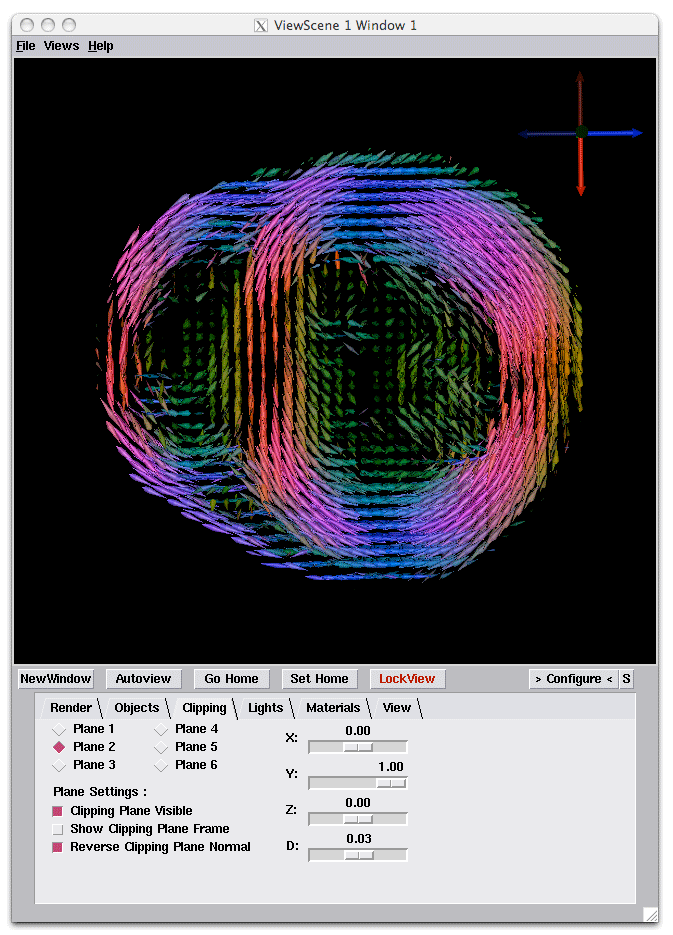
\includegraphics{IschemiaModelTutorial_figures/Vectors.png}}
\caption{Visualizing the Fiber Orientation of the Data}\label{fig:Vectors}
\end{figure}

In this example we will render Vectors as cones by selecting the {\bf Vector Display Type} in the UI and we use {\bf RGB Conversion} as the vector coloring. The latter option colors a vector red if it is aligned along the x-axis, green if it is aligned along the y-axis and blue for the z-axis. Depending on the orientation of the vector the red, green, and blue colors are mixed together to indicate the orientation. Also increase the the size of the {\bf VectorScale} to render glyphs that are larger. 

Also as these vectors represent the fiber direction, the actual direction they are pointing is arbitrary as they could just as well point in the opposite direction. It is the line the vectors are pointing along that matters in this case. To make the vectors point in both directions, set the option {\bf Render bidirectionally}.

The final image that is rendered is displayed in figure~\ref{fig:Vectors}. In this image we applied the slicing from the previous section, to highlight the fibers in a cross section through the left ventricle of the heart. By combing the networks examined in this tutorial one can visualize the different aspects of the data.


%---------------------------------------------

\chapter{Building a Tetrahedral Mesh}

\begin{introduction}
Scope: Isosurface - FairMesh - ResampleMesh - InterfaceWithTetGen -  Visualizing Meshes 
\end{introduction}

\section{Building a Tetrahedral Mesh}

In order to build a physical model out of the imaging data, we need to generate a computational mesh. In this example we describe an easy way of generating a tetrahedral mesh using isosurfaces. To build an elementary tetrahedral mesh, generate the network that is depicted in figure~\ref{fig:BuildMesh}. This network introduces two new modules called {\bf InterfaceWithTetGen} and {\bf WriteField}. 

\begin{figure}
\scalebox{0.65}{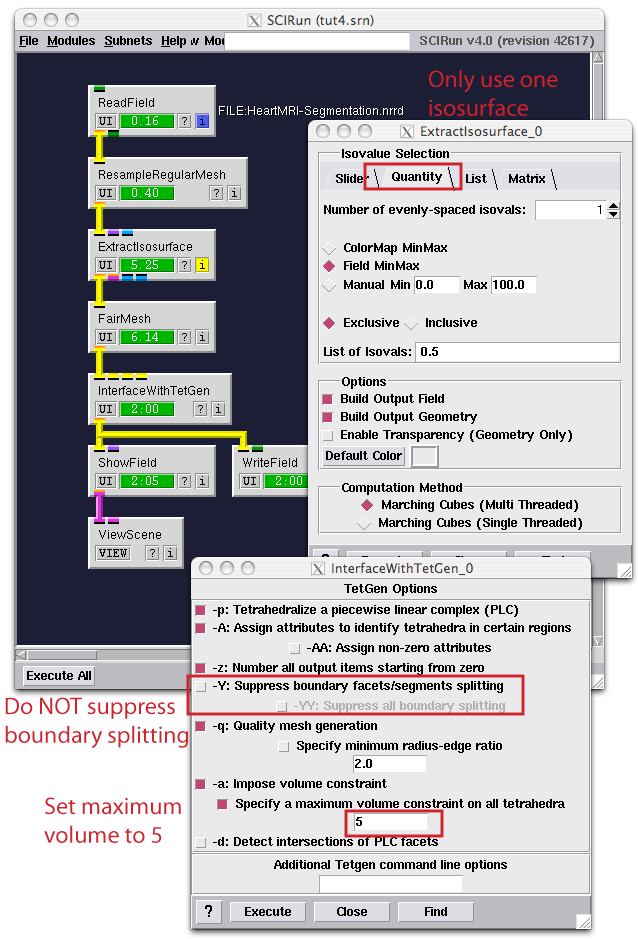
\includegraphics{IschemiaModelTutorial_figures/BuildMesh.png}}
\caption{Network for building a Tetrahedral Mesh}\label{fig:BuildMesh}
\end{figure}

The {\bf InterfaceWithTetGen} module lets SCIRun communicate with TetGen for generating a tetrahedral mesh. This module takes a triangular mesh as input and performs a constrained Delaunay Tetrahedralization and output a full volemtric mesh that consists of tetrahedral elements. In order to for tetrahedralization to succeed the isosurface generated by \textbf{ExtractIsosurface} needs to be smoothed. We use the {\bf FairMesh} module for this again. 

When opening the {\bf UI} of the  {\bf InterfaceWithTetGen} module, one can select out of a range of options to generate a mesh. The three options that are of interest in generating a computational tetrahedral mesh for this problem are the {\em -Y}, {\em -q}, and the {\em -a} option in the {\bf UI}. The {\em -Y} option lets the user decide whether additional vertices are to be inserted into the outer boundary. Suppressing splitting of the boundary facets often generates lower quality elements at the boundary, and forces TetGen to do far more computations, so in this example we switch it off. The next flag {\em -q} enforces quality of the elements, one can specify a lower ratio for a better quality. Normally enforcing a higher quality comes at the price of a longer computation and more elements. We keep this at its default setting. The final flag that is of interest is the {\em -a} flag that allows the user to specify the size of the elements. Besides element quality, element size is an important parameter for computing electromagnetic fields. Without a volume constraint the delaunay tetrahedralization will enforce the largest size elements it can fit within the interior of the mesh. As we do not want that in this case, we supply a volumetric maximum. In this case a value of 5 is reasonable value.

In this network, instruct the {\bf ReadField} module to read the file \textbf{HeartMRI-Segmentation.nrrd};
the \textbf{ResampleRegularMesh} module can keep its default settings. The reason for this module being added to the pipeline is reduce the number of elements in the segmentation, so that the example can be computed within a time frame of minutes in stead of hours. The {\bf ExtractIsosurface} module should be set to the {\bf Quantity }tap and we should be computing only one isosurface. The {\bf InterfaceWithTetGen} module options should be set as indicated in figure~\ref{fig:BuildMesh}. Finally, the {\bf WriteField} module should contain a name of a file that will be used to save the mesh, so we do not need to recompute for in the rest of the chapters. Supply a filename in the {\bf UI} of the module and press {\bf Set} to set the name of the file that will be written. Also open up the {\bf ShowField} module and disable the {\bf Show Nodes} and {\bf Show Edges}, although SCIRun can renderer these without any problems.

After pressing {\bf Execute All} to execute all modules allow for a few minutes for the model to build. As TetGen is running as an external library, we do not have a good estimate of how long it takes to render the mesh, hence even while the progress bar in the module is not moving progress is made and SCIRun will return within a several minutes and display the mesh. Use the slicing planes to examine the mesh (see figure~\ref{fig:ResultingMesh}).

\begin{figure}
\scalebox{0.5}{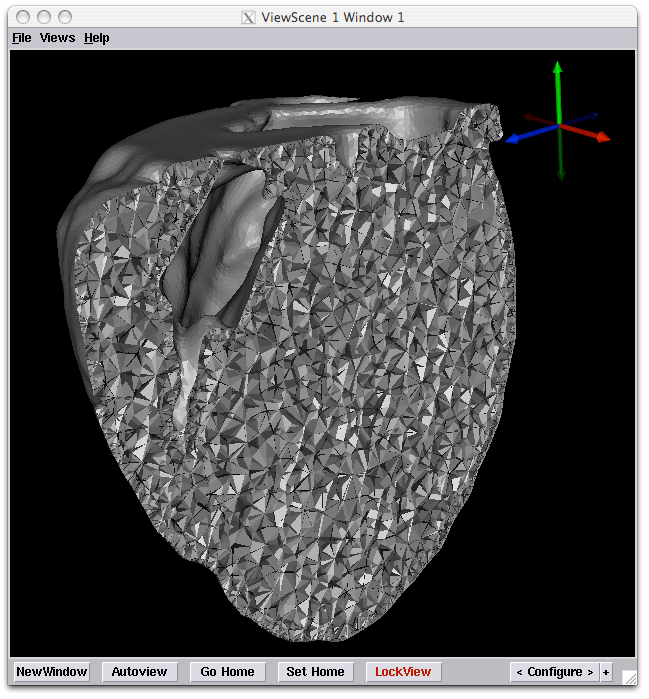
\includegraphics{IschemiaModelTutorial_figures/ResultingMesh.png}}
\caption{Image of the Tetrahedral Mesh}\label{fig:ResultingMesh}
\end{figure}

%---------------------------------------------  

\chapter{Tensors and Conductivities}

\begin{introduction}
Scope: SignedDistanceField - CalculateFieldData - Bundles - Mapping FieldData
\end{introduction}

\section{Creation of Model Parameters}

The next step in building the simulation is the creation of the model parameter spaces. In this example the model is defined by the conductivities of the intracellular and extracellular spaces as a function of space and the transmembrane potential as a function of space. 

To generate these model spaces we start with a clean canvas, and add a {\bf ReadField} module to read the mesh that was generated in the previous chapter. The full network for generating the model is outlined in figure~\ref{fig:BuildSimulationModel} with Figures~\ref{fig:BuildSimulationModel2}-\ref{fig:BuildSimulationModel4} detailing the setting of the various {\bf UIs}. Only those modules that need modifications to the default settings are listed in the figures.

This network starts by loading the previously generated mesh, and also loads the perfusion bed dataset and the fiber orientation dataset. All these three datasets are loaded at the top of the network. This data serves as material to build the heart specific models.

In the upper left corner of the network the perfusion bed dataset is loaded. The first step is to downsample the data by a factor 2 to make the computations more interactive for this tutorial. The next step is the extraction of the isosurface that defines the boundary of the ischemic zone. This boundary subsequently fed into the {\bf FairMesh} module to smooth out discretization effects, leaving a relative smooth definition of the ischemic border zone. This definition of the border zone is used for two purposes: (1) the definition of the transmembrane potential as a function of space and (2) the definition of the conductivity which changes as a function of space.

\begin{figure}
\scalebox{0.6}{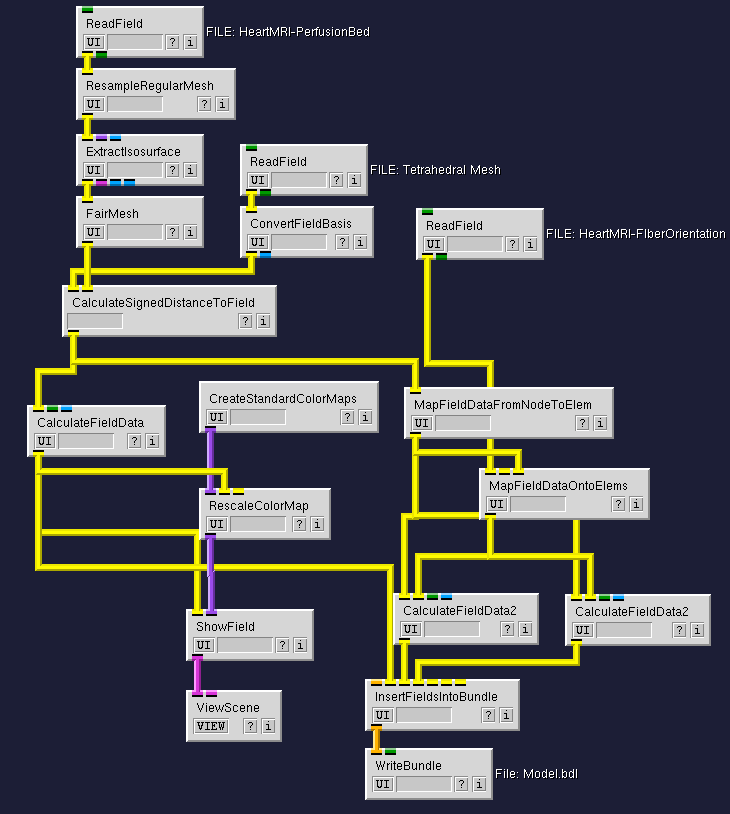
\includegraphics{IschemiaModelTutorial_figures/BuildSimulationModel.png}}
\caption{Full network for building extracellular, intracellular conductivity fields and the transmembrane potential fields}\label{fig:BuildSimulationModel}
\end{figure}

In order to define a volumetric function based on a surface we compute the distance to the surface for each node located in the mesh. As the ischemic zone is a closed volume we can use the {\bf CalculateSignedDistanceToField} module to determine the distance of each node to the surface. In this case a positive distance is rendered for each node inside the ischemic zone and a negative distance is rendered for each node outside of the surface. Although the computation of the distance fields for unstructured grids is generally a slow operation, the SCIRun code inside the module uses a parallel algorithm that should solve this distance field with a timeframe of less than a minute. However note that when the objects get more complex this operation can be relatively slow.

Below the  {\bf CalculateSignedDistanceToField} module, the distance field is inserted into the {\bf CalculateFieldData} module. The latter module evaluates a mathematical expression based on the data of the field. In this case we define a function that blurs the transmembrane potential based on the distance to the border zone. As the distance is signed we define the transmembrane potential inside the ischemic zone as -15 mV and the potential outside of the ischemic zone as +15mV, with the border zone at 0 mV. In this bidomain simulation we have altered the actual transmembrane potential to be centered around 0mV for convenience. As the choice of a reference potential does not alter the induced currents, the choice of the reference membrane potential does not matter. However if one wanted to one can add easily an additional term to equation.

\begin{figure}
\scalebox{0.5}{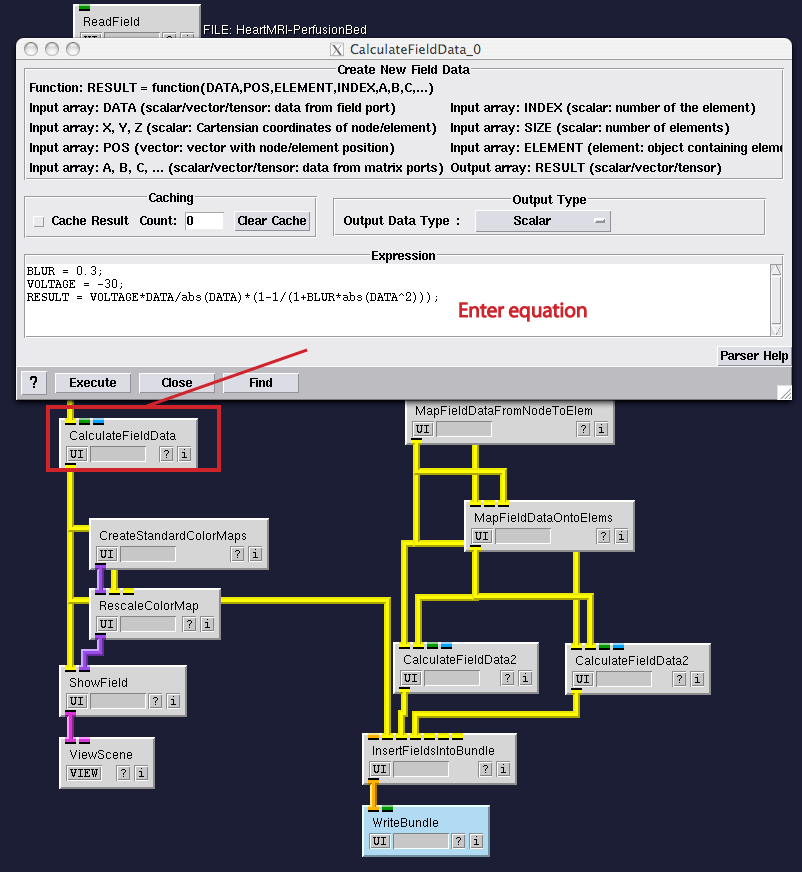
\includegraphics{IschemiaModelTutorial_figures/BuildSimulationModel2.png}}
\caption{UI settings of modules}\label{fig:BuildSimulationModel2}
\end{figure}

The equation displayed in figure~\ref{fig:BuildSimulationModel2} was chosen arbitrary to reflect a smooth transition of the transmembrane potential. The function here just indicates one of many functions that could have been chosen, as we are still in the process of actually determining what the shape of the ischemic border zone is. The equations displayed in the figure show various of the features of the built-in mathematical expression parser. It can parser a set of equations and one can define an arbitrary amount of additional parameters. The grammar of the parser requires that you separate each expression by a semi colon. Currently only expression as supported by the parser and no functions, loops, or conditional statements are supported.

\begin{figure}
\scalebox{0.5}{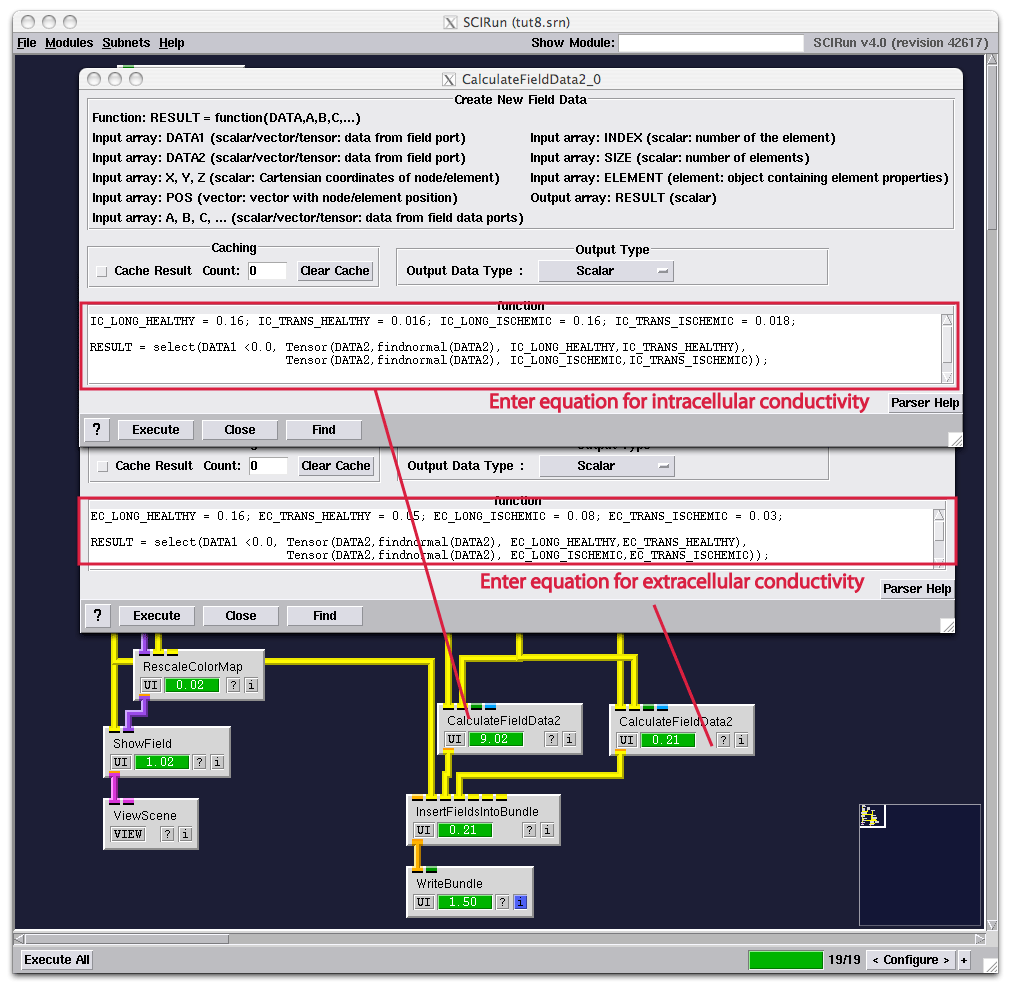
\includegraphics{IschemiaModelTutorial_figures/BuildSimulationModel3.png}}
\caption{UI settings of modules}\label{fig:BuildSimulationModel3}
\end{figure}

The {\bf CalculateFieldData2} module, which is based on the same mathematical expression parser, is used to generate the conductivity tensors as well. In figure~\ref{fig:BuildSimulationModel3} the example functions for these conductivities are given. Note that we use two input fields here and hence the function now is function of two spatial varying parameters. In this case we as a special function called {\bf select} which treads the first argument as a boolean expression and based on the outcome decides to evaluate the first or the second argument. This in a sense adds a conditional statement to the math parser. 



One difference with the function for the transmembrane potential is that the data now has to be located at the centers of the elements, as the Finite Element computations are currently restricted to conductivities defined for an element. In order to translate the distance field from a representation on nodes to a representation onto elements, we use the {\bf MapFieldDataFromNodeToElem} module. This module by default interpolates the data using a linear scheme to the center of each element of the mesh. 

\begin{figure}
\scalebox{0.45}{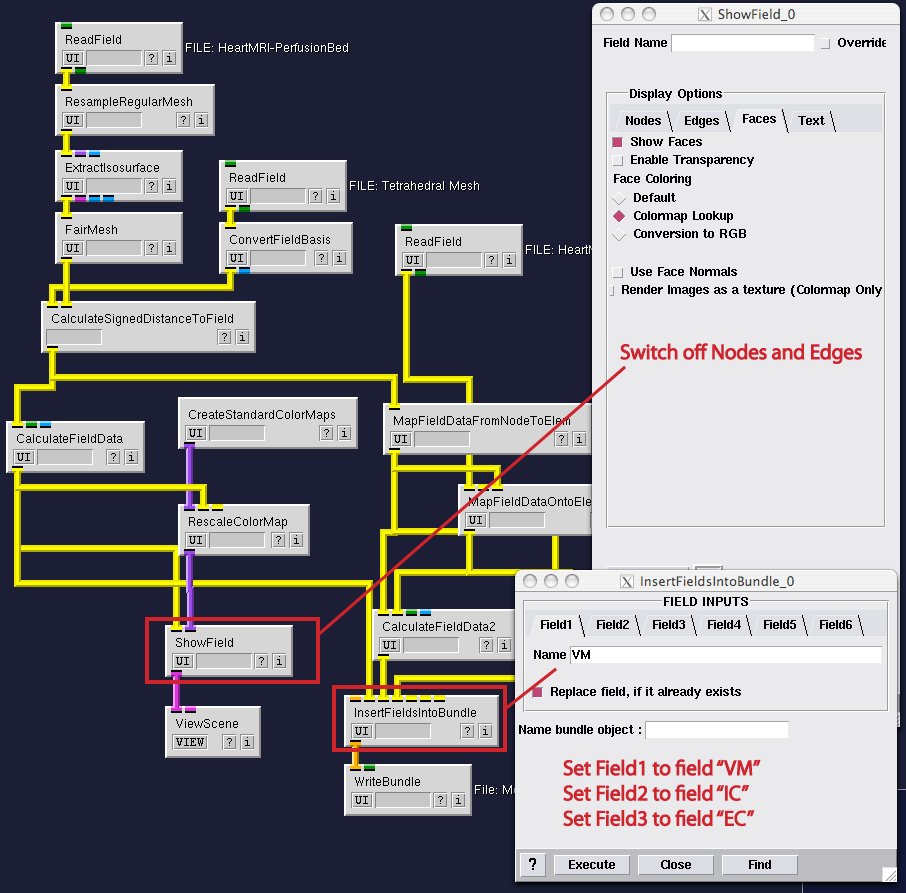
\includegraphics{IschemiaModelTutorial_figures/BuildSimulationModel4.png}}
\caption{UI settings of modules}\label{fig:BuildSimulationModel4}
\end{figure}

The transformation of the fiber orientation data is a bit more complex as it is located inside a different mesh. In order to map data from one mesh type to another mesh type, two special modules have been designed to help with mapping data from one mesh to another mesh, namely {\bf MapFieldDataOntoNodes} and {\bf MapFieldDataOntoElems}. In this case the latter module is used. By default the mapping of data onto elements is performed by choosing a range of sampling points inside each element and find the interpolated value for each location. The values are subsequently consolidated by averaging them. In case the user wanted a different integration scheme for the data, several methods are available for defining the data in the original, a variety of sampling schemes is available and several methods are available for combining the resulting values. In this case we use the default settings as they should render a good enough result.



The mapped distance field and fiber orientation are then used to compute the conductivity tensor. Within the math expression parser a full range of functions is available for defining the Tensor, in this case the first input into the Tensor function is the first eigenvector and the two subsequent scalars are the conductivity along this first axis, and the next one is the conductivity across. A second eigenvector would be permitted as well by defining two input vectors and three conductivity scalars. However for cardiac tissue only the conductivity ratio across versus along the myocardial fiber is known. It is assumed that across the fiber in both directions one has the same conductivity. 

The last part of the network introduces a new concept called the {\bf Bundle}. A bundle is no more than a collection of Fields and other objects that are stored by name. The advantage of bundling data is that one can store all the fields into one file. Which makes it easier to maintain the simulation data, as well as that it saves diskspace when components use common structures like an underlying mesh. (see figure~\ref{fig:BuildSimulationModel4})

To generate a bundle the {\bf InsertFieldsIntoBundle} module assigns each of the input ports to a new name in the bundle. In this case we choose the names enquote{VM}, enquote{IC} and enquote{EC} for the transmembrane potential, the intracellular conductivity, and the extracellular conductivity respectively. The bundle subsequently saved on disk for the simulation network of the next chapter.

\begin{figure}
\scalebox{0.5}{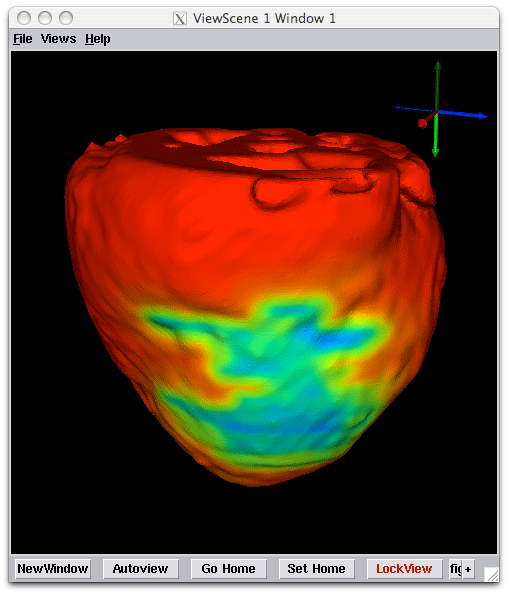
\includegraphics{IschemiaModelTutorial_figures/ModelOfVM.png}}
\caption{Visualization of assumed transmembrane potentials}\label{fig:ModelOfVM}
\end{figure}

Finally a small portion on the bottom left of the network is dedicated to displaying the transmembrane potential. This part of the network uses the modules from previous chapters to do generate a visualization of how the transmembrane potential looks like. Try for instance altering the \enquote{BLUR} parameter in the calculator module to see the effect of the blurring. An example of the output is given in figure~\ref{fig:ModelOfVM}.

%---------------------------------------------  

\chapter{Finite Element Modeling}

\begin{introduction}
Scope: BuildFEMatrix - ExtractIsosurfaceByFunction - Bundles - SolveLinearSystem - ApplyMappingMatrix -GetFieldData - SetFieldData
\end{introduction}

\section{Creating The Simulation}

We start with the bundle generated in the previous chapter. This bundle contains all the fields for running the simulation. To run the simulation build the network as depicted in figure~\ref{fig:SimulationNetwork}. Figure~\ref{fig:SimulationNetwork2}-\ref{fig:SimulationNetwork5} display the settings required in each of the module {\bf UI} menus. The modules that are not highlighted in these figures use the default settings of these modules.

The underlying idea of the this network is to solve the following equation :
\begin{equation}\label{eqn:bidomain}
	-(\nabla \cdot (\Sigma_i + \Sigma_e ) \nabla \phi_e) = \nabla \cdot \Sigma_i \nabla \phi_m
\end{equation}

\noindent in which $\Sigma_i$ and $\Sigma_e$ are the intracellular and extracellular conductivity tensors and $\phi_m$ is the transmembrane potential and $\phi_e$ is the extracellular potential. In this network the transmembrane potential $\phi_m$ is assumed to be the quantity that is known and the network computes the extracellular potentials $\phi_e$  that are actually measured in experiments. Hence, based on a proposed transmembrane potential, this network now computes the extracellular potentials.

\begin{figure}
\scalebox{0.6}{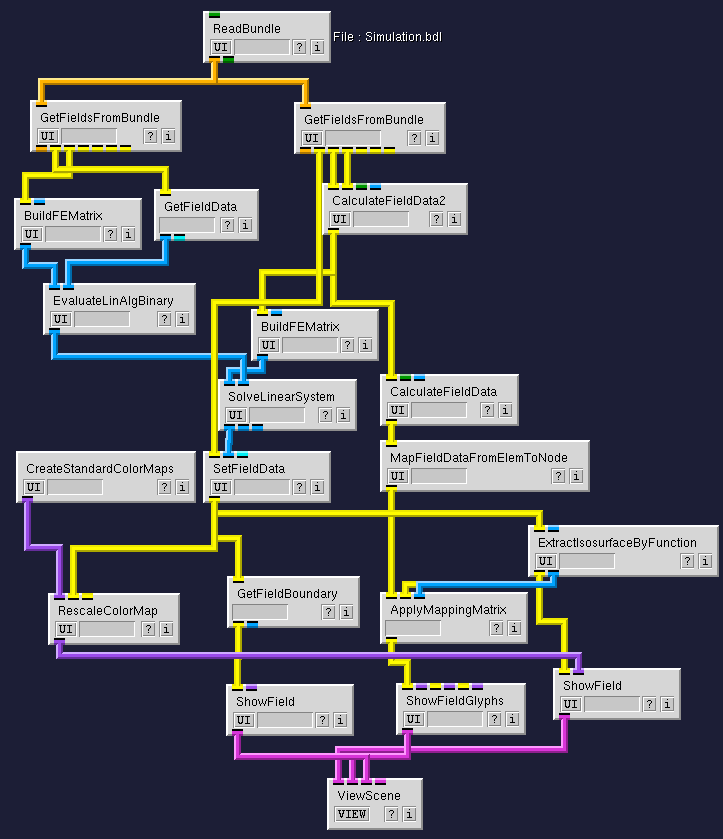
\includegraphics{IschemiaModelTutorial_figures/SimulationNetwork.png}}
\caption{Full network for running simulation}\label{fig:SimulationNetwork}
\end{figure}

At the top of the network the bundle is split in two, one part is used to create the right-hand-side of equation~\ref{eqn:bidomain} and the other part is used to compute the left-hand-side. As seen in equation~\ref{eqn:bidomain}  the left-hand-side depends on the summation of the intracellular and extracellular tensors. The module {\bf CalculateFieldData2} is used to sum the values of the intracellular and extracellular conductivity fields for each location. The output of this module is subsequently fed into the {\bf BuildFEMatrix} which builds the stiffness matrix for the Poisson equation. This stiffness matrix can be viewed as the discretization of the anisotropic Poisson equation and hence it is the numeric equivalent of the $\nabla \cdot (\Sigma_i + \Sigma_e ) \nabla$  operator.

The modules to the left of the creation of the stiffness matrix actually compute the right-hand-side vector. This is done again by using the {\bf BuildFEMatrix} module to generate the numerical operator  $\nabla \cdot (\Sigma_i ) \nabla$ and multiplying this with the values from the transmembrane potential field. As the output of the  {\bf BuildFEMatrix} module is matrix (blue pipe), the data inside the field needs to be represented as a vector. This is accomplished by the {\bf GetFieldData} module that strips the data from the nodes in the field and inserts it into a column matrix. In order to now obtain the right-hand-side vector we need to multiply the column vector with the matrix. The latter is accomplished by the {\bf EvaluateLinAlgBinary} module. 

\begin{figure}
\scalebox{0.5}{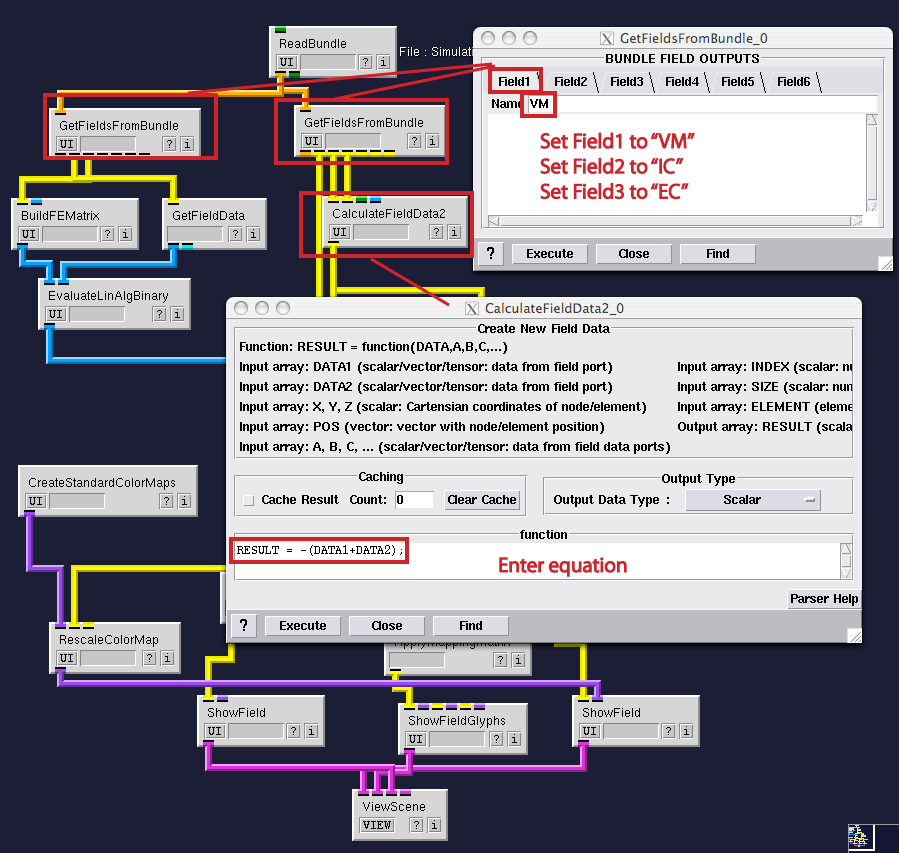
\includegraphics{IschemiaModelTutorial_figures/SimulationNetwork2.png}}
\caption{UI settings of modules}\label{fig:SimulationNetwork2}
\end{figure}

Both the stiffness matrix and the right-hand-side vector now form a linear system that needs to be solved to obtain the extracellular potentials. The {\bf SolveLinearSystem} module solves the linear system using in iterative solver. The details of the solver can be entered in the {\bf UI} of this module. Once the linear system is solved the solution contained in a column vector is reinserted into the field using the {\bf SetFieldData} module. An example of a reasonable number of iterations is given in figure~\ref{fig:SimulationNetwork3}.
Everything below this module in the network is used for visualizing the data which is described in the next section.

\begin{figure}
\scalebox{0.5}{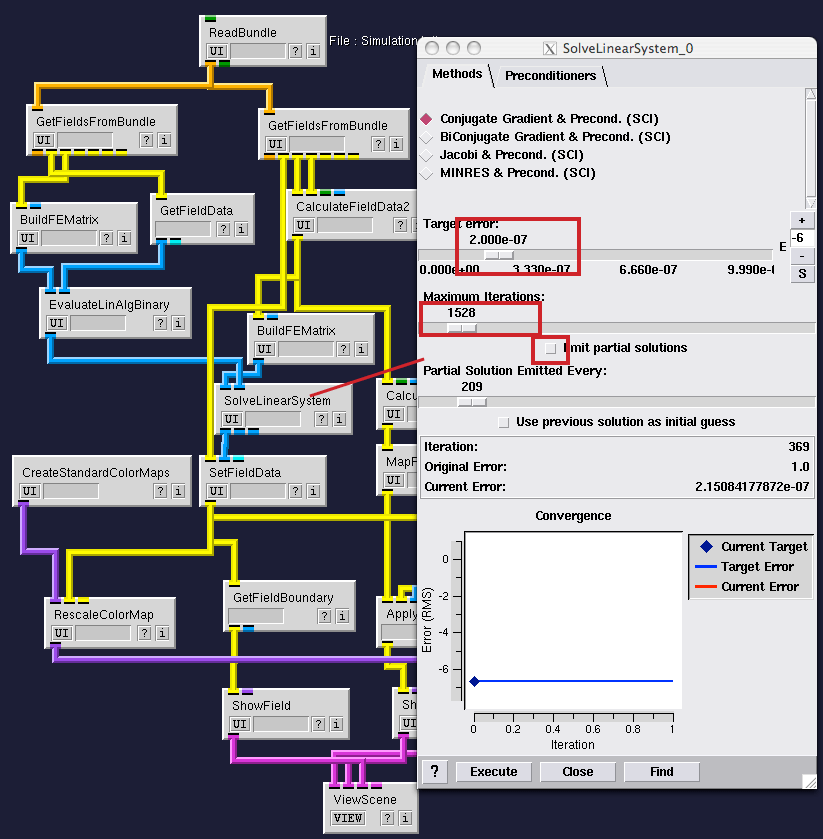
\includegraphics{IschemiaModelTutorial_figures/SimulationNetwork3.png}}
\caption{UI settings of modules}\label{fig:SimulationNetwork3}
\end{figure}

\section{Visualization of Simulation Results}

In order to study the effect of anisotropy on the extracellular potentials we look at a certain cross section of the model. In order extract a cross section we use the {\bf ExtractIsosurfaceByFunction} module. This module lets the user specify a function and subsequently extracts an isosurface of this function and projects the data back
onto this surface. In this case we use the function {\em RESULT=Y;} which will generate cross sections in the XZ-plane. However displaying the data without the underlying
fiber structure is of no use, therefore we can reconstruct the fiber orientation from the tensor data sending it through the calculator module again and extracting the first eigenvector using the {\it eigvec1()} function. The data is subsequently moved to the elements of the mesh.
\begin{figure}
\scalebox{0.45}{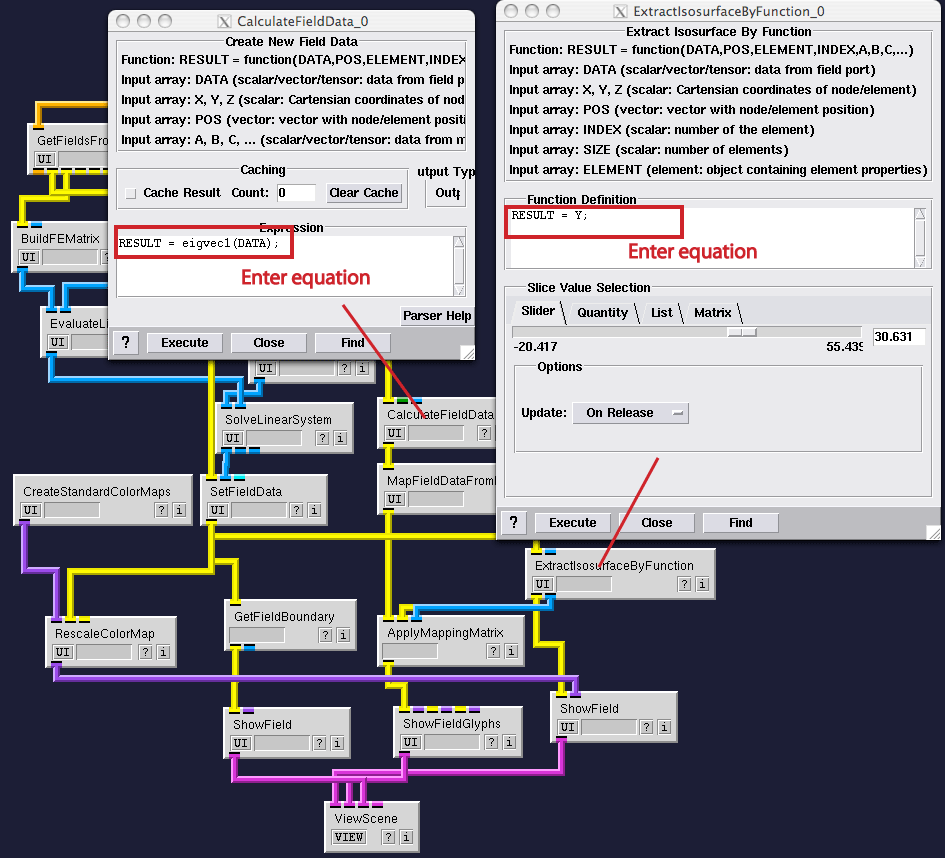
\includegraphics{IschemiaModelTutorial_figures/SimulationNetwork4.png}}
\caption{UI settings of modules}\label{fig:SimulationNetwork4}
\end{figure}

To efficiently project the data onto the same mesh as the data, we use the {\bf ApplyMappingMatrix} module, this allows to quickly copy the data from one mesh to another mesh if the operation that generated the new mesh computed a so called mapping matrix. In this case the {\bf ExtractIsosurfaceByFunction} did compute such a mapping matrix and we will be able to project the data onto the same grid. As often in SCIRun there are many ways to do the same thing, we could just as well have used the {\bf MapFieldDataOntoElems} module to accomplish the same. 

\begin{figure}
\scalebox{0.45}{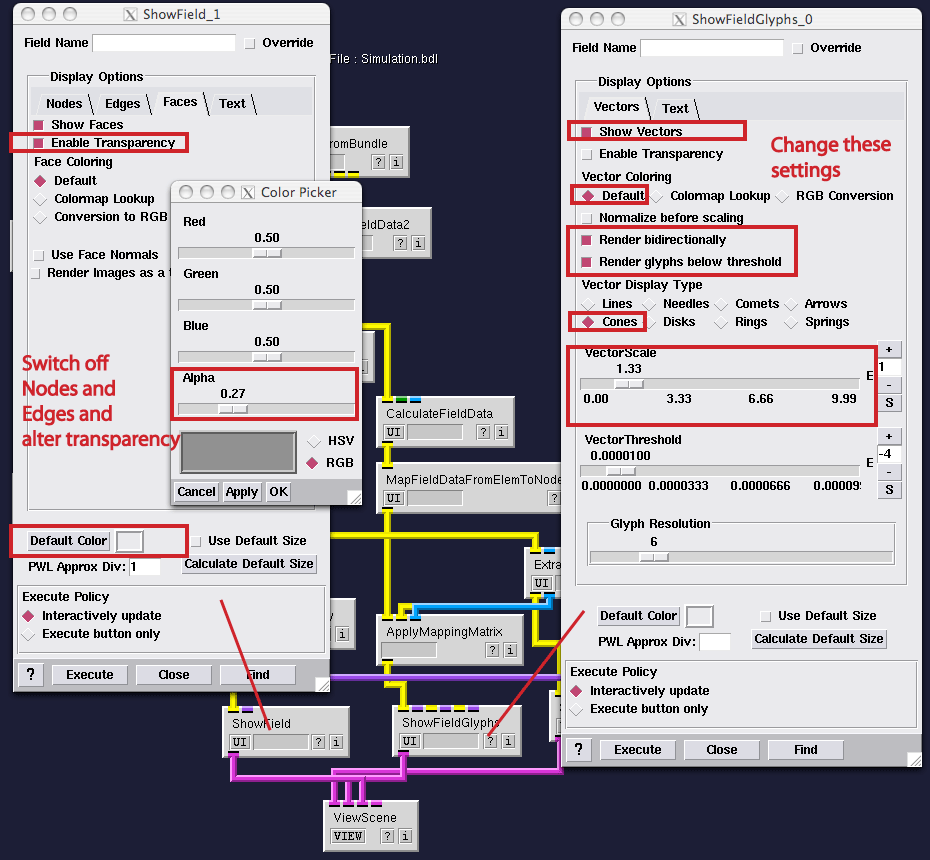
\includegraphics{IschemiaModelTutorial_figures/SimulationNetwork5.png}}
\caption{UI settings of modules}\label{fig:SimulationNetwork5}
\end{figure}

Finally the vectors and the data are combined into one viewer. In order to render a sense or orientation we also render a transparent shell of the mesh. The {\bf GetFieldBoundary} module extracts the outside of any mesh. In this case it renders the outer surface of the model. The {\bf ShowField} module can be setup so it renders a transparent version of the mesh boundary. Disable the display of nodes and edges and alter the {\bf Default Color} as indicated by figure~\ref{fig:SimulationNetwork5}. By  altering the Alpha value the mesh can be made far more transparent, so to highlight the cross section more clearly. Also increase the scale of the vectors so they become clearly visible.

\begin{figure}
\scalebox{0.45}{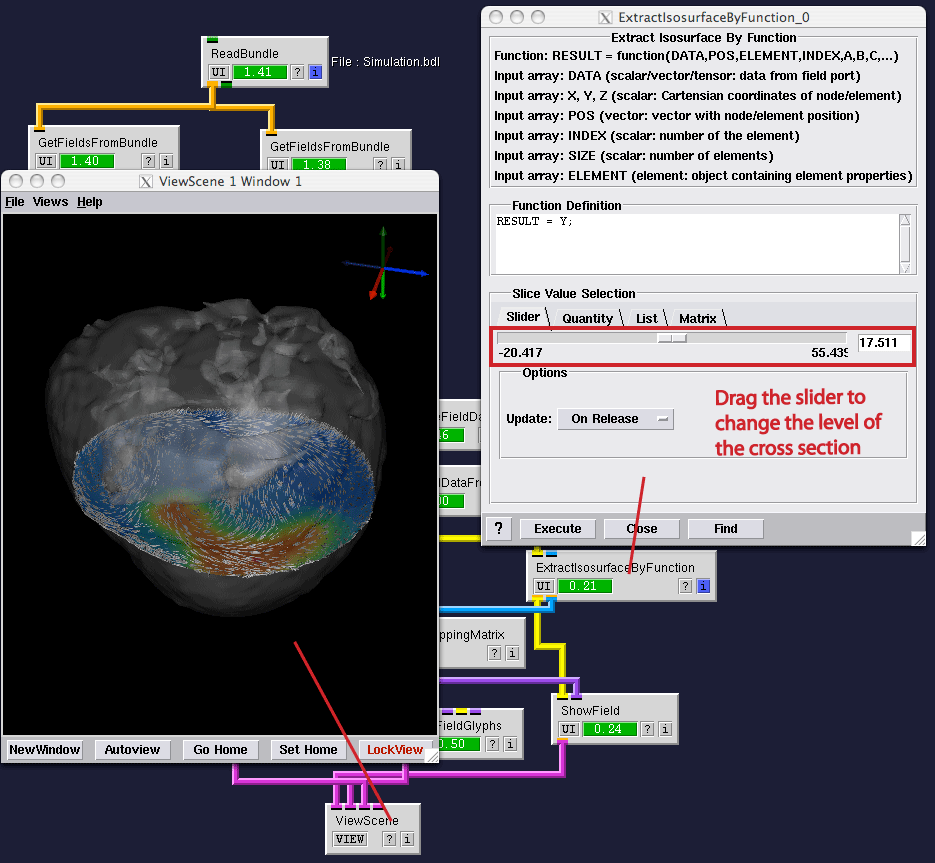
\includegraphics{IschemiaModelTutorial_figures/SimulationNetwork6.png}}
\caption{Visualizing Results}\label{fig:SimulationNetwork6}
\end{figure}

Finally the {\bf ViewScene} module displays a result that show that the potentials tend to stretch along the fiber orientation, as can be viewed by the results indicated in figure~\ref{fig:SimulationNetwork6}.

\end{document}

